\chapter{Mobilitātes Modeļi}\label{sec:mobilityModels}
Mobilitātes modelis ir noteikumu kopa, kas nosaka mobilas vienības trajektoriju \cite{tuduce}. Modelim jāatbilst sekojošiem  kritērijiem:
\begin{itemize}
\item jābūt iespējai apvienot kopā n modeļus un izveidot tādu pašu lielāka izmēra modeļus
\item jābūt mainīgiem lielumiem, kurus mainot var izveidot dažādus mobilitātes  scenārijus
\item modelim jābūt stacionārai
\item modelim nepieciešams nekorelēt
\end{itemize}

Pamatmetode ar kuru pēta ekspromta tīklu darbību un procesus ir datorsimulācija (turpmāk simulācija). Simulācijai ir vairākas būtiskas priekšrocības: iespēja identiski atkārtot scenāriju, iespēja izolēt noteiktus parametrus un iespējams variēt dažādus tīkla raksturlielumus. Mobilo Ad Hoc un WSN tīklu simulācijā galvenie faktori ir tīkla topoloģija un mezglu kustība, kas ietekmē pētāmā tīkla parametrus. Tīkla topoloģija nosaka mezglu sākotnējo izvietojumu, savukārt mobilitātes modelis nosaka mezglu kustību tīklā. Mezglu mobilitātes modelis visvairāk ietekmē maršrutēšanas protokola darbību. Simulācijas rezultāti, kas iegūti ar nekorektu mobilitātes modeli izveido nepareizu priekšstatu  par protokolu darbību un par tīklā notiekošiem procesiem.

Mobilitātes modeļi tiek uzskatīti par vienu no lielākajām problēmām mobilo ekspromta tīklu simulācijas jomā \cite{tuduce}. Reālas pasaules lietotāju uzvedības modelēšana ir sarežģīts uzdevums un bieži rodas nepieciešamība izvēlēties kompromisu starp modeļa sarežģītību un precizitāti. Viens no paņēmieniem ir novērot mobilitātes modeli (tā rakstu) reālā sistēmā. Tomēr metode nav pilnībā efektīva, jo tā atspoguļo tikai vienu kustības scenāriju, kuru nav iespējams vispārināt. Turklāt, šādi modeļi neatbilst iepriekš minētajam kritērijam, proti modelim ir jābūt stacionārām, jo lietotāju kustība un daudzums ir atkarīgs no diennakts laika. Piemēram, lielveikala apmeklētāju skaits diennakts laikā  var svārsties no 0 apmeklētājiem naktī, līdz simtiem apmeklētāju pīķa stundās. Risinājums ir mākslīgie modeļi (synthetic models), kas plaši tiek  pielietoti daudzos pētnieciskos projektos. Vairums no šobrīd visplašāk sastopamajiem mākslīgajiem modeļiem ir aprakstīti Camp darbā \cite{camp}. Šajā nodaļā tiks apskatīti trīs visbiežāk pielietojamie modeļi: \acf{RWMM}, \acf{RDMM} un \acf{OMM}. Šie modeļi ir pieejami \acl{NS-2} un GloMoSim datorsimulāciju programmās.

\begin{figure}[htb!]
\begin{minipage}[t]{0.45\linewidth}
\centering
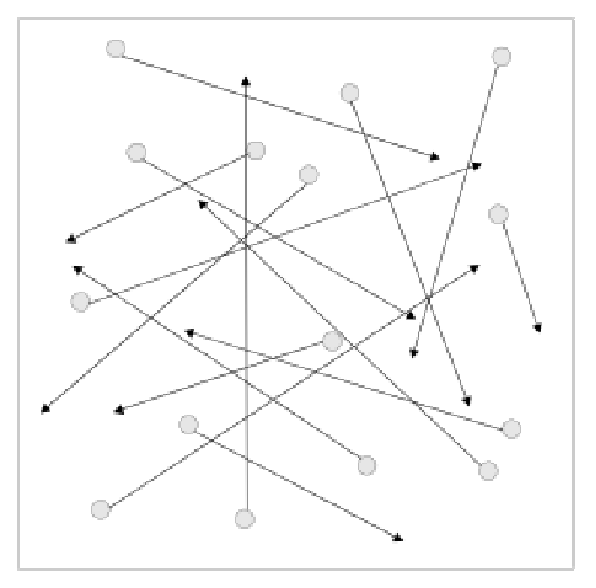
\includegraphics[scale=0.45]{./graph/RWMM1}
\caption{Gadījuma maršrutpunktu mobilitātes modelis (RWMM)} \label{fig:rwmm}
\end{minipage}%
\hspace{0.5in}
\begin{minipage}[t]{0.45\linewidth}
\centering
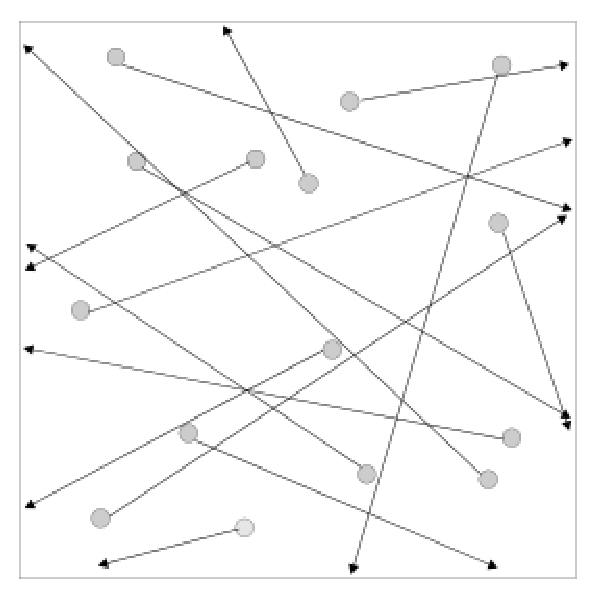
\includegraphics[scale=0.45]{./graph/RWMM2}
\caption{Gadījuma virzienu mobilitātes modelis (RDMM)} \label{fig:rdmm}
\end{minipage}
\end{figure}

\section{Mobilitātes modeļu raksturlielumi}
Ja tīklu apskata no simulācijas viedokļa, tad mobilitātes modeļi būtībā atšķiras pēc mezglu sākotnējas izvietošanas tīkla laukumā $S^{2}$ un ar mezglu izmaņu simulācijas laikā. Lai modeli raks-turot matemātiski, izmanto telpisko mezglu izvietošanu laukumā. Lai simulācijas mērķis būtu ar pēc iespējās reālistisku scenāriju, tad ir jāņem vērā arī: mezglu kustības ātrumu, savienojuma ilgumu, mezglu izkliedi un to blīvumu tīkla laukumā.

\subsection{Atkarība starp tīkla laukumu un mezglu ātrumu}
Sākuma mezglu izvietojums un ātrums nosaka vēlāko mezglu izvietojumu simulācijas laukumā. Turklāt izvietošanas un ātruma varbūtības sadalījums nepārtraukti mainās laika gaitā. To - kādā laika brīdī tīkls sasniegs savu 'līdzsvara' stāvokli, matemātiski var aprakstīt ar stacionāro sadalījumu \cite{navid}.

\subsection{Savienojuma ilgums}
Savienojuma ilgums ir laika periods starp savienojuma izveidi līdz tā izjaukšanai. Simulācijas vidējais savienojuma ilgums ir vidējais aritmētiskais no visiem savienojumiem, kas tiek izveidoti simulācijas laikā. Šis parametrs ir svarīgs jo mēdz gadīties, ka protokoli, kuriem ir nepieciešams platjoslas savienojums, nebūs spējīgi darboties īslaicīgā savienojuma dēļ.

Bieži vien simulāciju programmās tiek pieņemts, ka savienojums izveidojas tiklīdz mezgli ir viens otra uztveres diapazonā (attālums starp mezgliem $\leq$ \gls{r_link}). Reālajā dzīve tā nav, jo brīdī, kad mezgls konstatē elektromagnētiskā signāla klātbūtni, pirms komunikācijas uzsākšanas ar raidītājmezglu,  tam ir nepieciešams sinhronizēties. Piemēram, ierīcēm ar Bluetooth tehnoloģiju ir nepieciešamas aptuveni 10 sekundes, lai divi mezgli uztveres diapazonā izveidotu savienojumu. Ņemot vēra šo faktu, kā arī to, ka mezgli kustas ātri, pastāv ļoti augsta varbūtība gadījumam, ka $r_{link}$ attālumā atrodošies divi mezgli, kas ātri kustas pretējos virzienos, nevarēs izveidot savienojumu (pat ja kādā brīdī tie būs ļoti tuvu). Tas ir tādēļ, ka laiks, kas ir nepieciešams savienojuma izveidošanai ir lielāks par laiku, kurā tiek šķērsota distance $r_{link}$.

\subsection{Mezglu blīvums}
$A$ mezglā kaimiņ-mezglu blīvums ir mezglu skaits kas atrodas $A$ mezgla uztveres diapazonā. Tīklā, kur telpiskais sadalījums ir viendabīgs, vidējais kaimiņ-mezglu blīvums ir būtisks parametrs. Aprēķina pēc (\ref{eq:blivums}) formulas.

\subsection{Mezglu izkliede}
Mezglu blīvums arī saukts par telpisko blīvums, ir mezglam $A$ kaimiņ-mezglu skaits $y$ uz laukuma vienību, šos kaimiņus var sadalīt $i$ dažādās kārtās (\seename~\figurename. ~\ref{fig:topo}) un aprēķina kā $\rho_{s}=\frac{N}{A}$. Ja mezglu skaits pirmajā kārtā ir $k$, tas nozīme ka sadalījums $D(k)$ ļauj izvēlētajam mezglam $A$ izveidot $k$ skaitu savienojumu. Dalījums kārtās sniedz iespēju iegūt informāciju par to vai mezglam $A$ būs iespējams izveidot savienojumu vai nē. Jo augstāka mezglu izkliede tīklā, jo augstāka ir varbūtība, ka mezgls $A$ izveidos 0 savienojumu.


\section{Gadījuma maršrutpunktu mobilitātes modelis}
Gadījuma maršrutpunktu mobilitātes modelis (\acs{RWMM}) ir viens no vienkāršākajiem un arī visplašāk pielietojamais mobilo Ad Hoc tīklu simulēšanai. Gadījuma maršrutpunktu mobilitātes modelī katram mezglam ir noteikts izvietojums (\seename~\figurename.~\ref{fig:rwmm}). Pārraides laikā ātrums \gls{v} un kustības virziens nemainās. Mezgla kustības galamērķis ir nejauši izvēlēta vieta tīkla laukumā. Ātrums $v$ ir izvēlēts intervālā $(v_{min}, v_{max})$, neatkarīgi no mezgla sākotnējās pozīcijas un tā kustības galamērķa. RWMM minimālais ātrums $v_{min}$ var būt tikai pozitīvs skaitlis, pretējā gadījumā vidējais ātrums būs negatīvs lielums. Kad mezgls nonāk galamērķī, tas var izdarīt pārtraukumu uz nejauši izvēlētu laiku, vai arī turpināt kustību uz jauno galamērķi. Mezglam tiek piešķirts jauns galamērķis un jauns ātrums $v$ neatkarīgi no iepriekšējā ātruma, galamērķa un pārtraukuma izvēles. Simulēšanas procesā RWMM mezglu izvietojums un ātrums neatbilst vienveidīgam izkārtojumam. Novērots, ka stacionārs mezglu izkārtojums tiek koncentrēts ap tīkla centru (\seename~\figurename.~\ref{fig:rwmm}), kurā notiek aktīva mezglu kustība \citep{bett, navid}.

\section{Mobilitātes modeļa ietekme uz BER}
Mezglu mobilitāte var tikt raksturota ar  ātrumu $v$ un tā leņķi \gls{theta} (leņķis attiecībā pret horizontālo asi). Gadījuma maršrutpunktu mobilitātes modelī (\acs{RWMM}) ziņojuma pārraides laikā, divu pārraidē iesaistītu mezglu ātrums un kustības virziens paliek nemainīgs.
\subsection{Scenārijs ar RWMM un NRBS}
Tiek uzskatīts, ka daudzposmu maršrutā secīgie posmi ir neatkarīgie viens no otra. Katrā no diviem posmiem vienā un tajā pašā maršrutā, mezgla beigu pozīcija (savienojumā, kur tas ir uztvērējs) būs neatkarīga no tā paša mezgla pozīcijas nākošā posma sākumā (jaunajā savienojumā, kur tas ir raidītājs). Mezgli $n_{A}$ un $n_{B}$ ir mezglu pāris kurš veido savienojumu. Ziņojuma pārraides laikā abiem mezgliem ātrums un virziena leņķis ir konstantes, $(v_{A}, \theta_{B})$ un $(v_{B}, \theta_{B})$. Sākotnējā pozīcijā mezgli $n_{A}$ un $n_{B}$ atrodas $r_{link}$ attālumā. Att.~\ref{fig:dp} ilustrēts kā mainās savienojuma garums $r_{link}$ a) pārraides sākumā $t_{s}$ un b) pēc ziņojuma pārraides $t_{e}=t_{s}+t_{msg}$.

\begin{figure}[!htb]
\centering
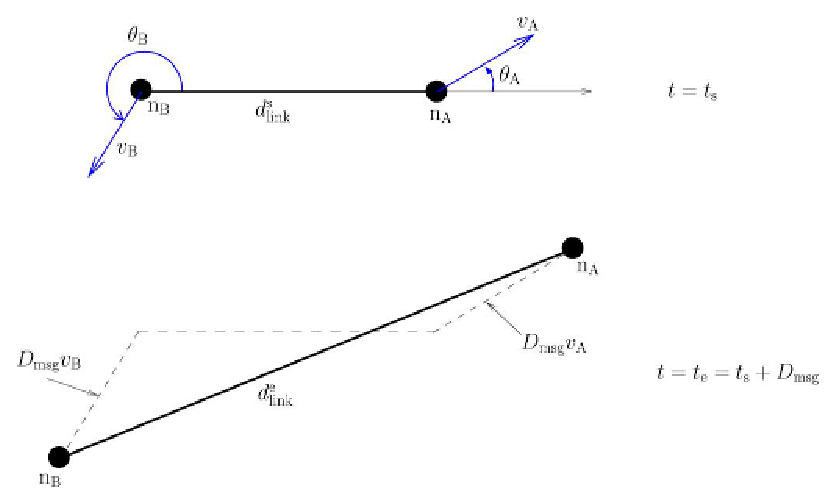
\includegraphics[scale=0.65]{./graph/dp}
\caption{Mezgla kustības trajektorija ar RWMM pie NRBS \cite{qoS_mobility}}
\label{fig:dp}
\end{figure}
Pielietojot kosinusu teorēmu posma garums $r_{link}^{e}$ laika bridī $t_{e}$ būs
\begin{align}
r_{link}^{e} &= \left[ r_{link}^{2} + t^{2}_{msg}(v^{2}_{A}+v^{2}_{B})-2v_{A}v_{B}t^{2}_{msg}cos(\theta_{A}-\theta_{B})+ \right. \nonumber \\
    &\qquad {}\left.	+2r_{link}t_{msg}(v_{A}cos\theta_{A}-v_{B}cos\theta_{B})\right]^{\frac{1}{2}}
\end{align}
Tātad, divu mobilu mezglu vidējais maršruta posma garums $\bar{r}_{link}$ ir vienāds ar $\bar{r}_{link}=\frac{1}{2}(r_{link}+r_{link}^{e})$. Lai aprēķinātu SNR pārraides laikā var izmantot (\ref{eq:snr}) formulu, aizvietojot $r_{link}$ ar $\bar{d}_{link}$. Pamatatšķirība ar statiska tīkla ir tā, ka $\bar{d}_{link}$ ir gadījuma lielums, kas ir atkarīgs no $(v_{A}, \theta_{A})$ un $(v_{B}, \theta_{B})$.

Vienkāršībai, tiek uzskatīts, ka katra mezgla kustības veids ir neatkarīgs no pārējiem mezgliem. Ziņojuma pārraides laikā daudzposmu maršruta $i$-tās posma ($i \in {1,\cdots ,\bar{n}_{h}}$), divu mezglu ātrums un kustības virziens ir $\zeta_{i}=(v_{i},\theta_{i},v_{i+1}, \theta_{i+1})$. Kur divi secīgi stāvokļi $(v_{B},\theta_{B})$ un $(v_{A}, \theta_{A})$ attiecas uz vienu un to pašu mezglu. Šis pieņēmums neietekmē savienojumu posmu skaitu daudzposmu maršrutā \cite{qoS_mobility}. Acīmredzams, ka $\bar{r}_{link} = r_{link}(\zeta_{i})$ un $i$-tā lēkuma BER būs $BER_{link}(\zeta_{i})$. Tādēļ daudzposmu maršruta galā $BER_{route}$ ar vidējo lēkumu skaitu $\bar{n}_{h}$ un pie $\zeta_{NRBS}=(\zeta_{1}, \cdots,\zeta_{\bar{n}_{h}})$ būs \cite{qoS_mobility}
\begin{equation}
BER_{route}(\zeta_{NRBS})=1-\prod_{i=1}^{\bar{n}_{h}}\left[1-BER_{link}(\zeta_{i})\right].
\end{equation}
Pie pietiekami liela realizāciju skaita $\eta$, $\zeta_{NRBS}^{j}=(\zeta^{j}_{1}, \cdots,\zeta^{j}_{\bar{n}_{h}}), j\in[1, \cdots,\eta]$ vidējais BER būs \cite{qoS_mobility}
\begin{equation}
BER_{route}=\frac{\sum_{j=1}^{\eta}BER_{route}\left(\zeta_{NRBS}^{j}\right)}{\eta}.
\end{equation}


\subsection{Scenārijs ar RWMM un RBS}
Pēc maršruta izveides, ziņojums 'plūst' caur iepriekš rezervētiem maršruta posmiem neatkarīgi no pārmaiņām tajā un mobilitātes iespaida. Att. ~\ref{fig:dpRBS} ilustrēta mezglu mobilitātes ietekme uz iepriekš rezervētu maršrutu. Attēlā, kad $t=t_{1}+5\times t_{msg}$ var redzēt, kā maršruts izliecas ap $n_{3}$ mezglu. Maršrutu iespējams pilnveidot izslēdzot $n_{3}$ no maršruta, jo mezgli $n_{2}$ un $n_{4}$ var komunicēt pa tiešo. Acīmredzams, ka - jo lielāks mezglu ātrums $v_{i}$, jo ātrāk notiks savienojuma posma pārrāvums.

\begin{figure}
\centering
\includegraphics[scale=0.40]{./graph/dpRBS.png}
\caption{Maršruta izmaiņas pārraides laikā ar RBS \cite{qoS_mobility}}
\label{fig:dpRBS}
\end{figure}

Tā kā RBS iepriekš rezervē mezglus visa maršruta garumā un tas nemainās visas pārraides laikā, tad mēs varam uzreiz aprēķināt visa maršruta garuma izmaiņas. Maršruts sastāv no $i$ savienojumiem posmā starp $n_{i}$ un $n_{i+1}$ mezgliem, ziņojuma pārraides laikā $t = t_{1}+(i-1)t_{msg}$, sākuma un beigu maršruta garumi var tikt izteikti\footnote{Balstīts uz pieņēmuma, ka starp diviem kaimiņ-mezgliem izplatīšanās laiks ir niecīgs, salīdzinot ar visa ziņojuma pārraides laiku. Šis pieņēmums ir patiess visa veida sensoru tīkliem, kuros veiksmīgi izveidoti savienojumi starp kaimiņ-mezgliem.}, kā \cite{qoS_mobility}:

\begin{align}
  r_{link}^{i,s} &= \left[ r_{link}^{2} + ((i-1)t_{msg})^{2}(v_{i}^{2} + v_{i+1}^{2})-2v_{i}v_{i+1}((i-1)t_{msg})^{2}cos(\theta_{i}-\theta_{i+1})+ \right.\nonumber \\
    &\qquad {} \left.  +2r_{link}(i-1)t_{msg}(v_{i}cos\theta_{i}-v_{i+1}cos\theta_{i+1})\right]^{\frac{1}{2}} 	\nonumber
\end{align}
\begin{align}
  r_{link}^{i,e} &=\left[ r_{link}^{2} + (it_{msg})^{2}(v_{i}^{2} + v_{i+1}^{2})- 2v_{i}v_{i+1}(it_{msg})^{2}cos(\theta_{i}-\theta_{i+1})+ \right.\nonumber \\
     &\qquad {} \left.  +2r_{link}i t_{msg}(v_{i}cos\theta_{i} - v_{i+1}cos\theta_{i+1}) \right]^{\frac{1}{2}}  \nonumber
\end{align}

Tātad, vidējo maršruta garumu var aprēķināt kā aritmētisko vidējo no sākuma un beigu garumiem $\bar{r}_{link}^{i} = (r_{link}^{i,s}+r_{link}^{i,e})/2$.

BER $i$-tā savienojuma posma beigas var izteikt izmantojot (\ref{eq:BER_routeProd}) formulu, aizvietojot $r_{link}$ ar $\bar{r}_{link}^{i}$, kas ir atkarīgs no $(v_{i}, \theta_{i})$ un $(v_{i+1}, \theta{i+1})$. Un vidējais maršruta posmu skaits ir $[\bar{r}_{link}^{1},\cdots, \bar{r}_{link}^{\bar{n}_{h}}]$, kas ir atkarīgs arī no realizēto mezglu kustībām $\zeta_{RBS} = [(v_{1},\theta_{1}),\cdots ,(v_{\bar{n}_{h}}, \theta_{\bar{n}_{h}})]$.

Vienkāršība laba tiek uzskatīts, ka katra mezgla kustības veids ir neatkarīgs no pārējiem mezgliem. Ziņojuma pārraides laikā daudzposmu maršruts ar $i$ savienojumiem ($i \in {1,\cdots ,\bar{n}_{h}}$) divu mezglu ātrums un kustības virziens ir $\zeta_{i} = (v_{i},\theta_{i},v_{i+1}, \theta_{i+1})$. Tādēļ daudzposmu maršruta galā $BER_{route}$ ar viduvēju lēkumu skaitu $\bar{n}_{h}$ un $\zeta_{RBS}$ būs \cite{qoS_mobility}

\begin{equation}
BER_{route}(\zeta_{RBS}) = 1-\prod_{i=1}^{\bar{n}_{h}-1}\left[1-BER_{link i}(\zeta_{i})\right].
\end{equation}

Pie pietiekami liela realizāciju skaita $\eta$, $\zeta_{RBS}^{j} = [(v^{j}_{1}, \theta^{j}_{1}), \cdots,(v^{j}_{\bar{n}_{h}}, \theta^{j}_{\bar{n}_{h}})], j\in[1, \cdots,\eta]$ vidējais BER būs
\begin{equation}
BER_{route}=\frac{\sum_{j=1}^{\eta}BER_{route}\left(\zeta_{RBS}^{j}\right)}{\eta}.
\end{equation}

% \emph{\textbf{As at the end of the previous section, the final expression for the route BER is given by (19).}}


\section{Gadījuma virzienu mobilitātes modelis}
Gadījuma virzienu mobilitātes modelī (\acs{RDMM}) mezglu sākotnējā izvietošana tīkla laukumā ir vienveidīga un paliek nemainīga visas simulācijas laikā. RDMM mezgli maina kustības virzienu un ātrumu ziņojuma pārraides laikā. RDMM modelī mezglu kustība ir neatkarīgi un viendabīgi sadalīta (\acs{iid}), kustības virzienu maiņa notiek 'nepārtraukti' (laikā nepārtraukts stohastisks process). Mezglu kustības virzienu maiņa notiek laika periodos. Katrā laika periodā mezglam ir noteikts ātrums $v_{m}$ un virziens. Laikā perioda garums ir gadījuma lielums $p$, kas ir eksponenciāli sadalīts ar lielumu $\lambda_{m}$. Absolūti nepārtrauktu sadalījumu (\acs{CCDF}) $F_{m}(p)$ var izteikt kā \cite{camp}
\begin{equation}
F_{m}(p)=exp(-\lambda_{m}p)
\end{equation}

Katrā laika periodā kustības virziens (intervālā $[0, 2\pi)$) un ātrums $[v_{min}, v_{max}]$ ir vienmērīgi sadalīti. Ātrums, kustības virziens un perioda garums ir neatkarīgi katrā laika periodā. Turklāt, kad mezgls sasniedz šūnas robežu, tad mezgla kustības virziens tiek mainīts uz diametrāli pretējo, bet ātruma modulis paliek nemainīgs. Minimālais ātrums $v_{min}$ var būt nulle un pārtraukumā tas ir nulle.


\section{Šķēršļu mobilitātes modelis}
Šķēršļu mobilitātes modelis (\acs{OMM})  ir reālistisks mobilitātes modelis, kurā tīkla laukumā iekļauti šķēršļi \cite{jabra,jabras}. Šķēršļi ierobežo gan mezglu kustību, gan to signālu pārraidi (\seename ~\figurename. ~\ref{fig:omm1}). \acs{OMM} kustības trajektoriju izveidošanai izmanto Voronoi trajektorijas aprēķinu (Voronoi path computation) metodi\cite{aur}. Šķēršļu mobilitātes modelī šķēršļiem ir poligona forma, kas Voronoi diagrammu dala vienādās daļās (\seename ~\figurename. ~\ref{fig:omm2}). Tas dod iespēju aprēķināt Voronoi dalījumu skaitu simulācijas laukumā. Katrs Voronoi dalījums, kuram nav šķēršļa, tiek uzskatīts par iespējamo kustības trajektoriju.
 Mezgli var būt nejauši izvietoti segmentos izmantojot īsākā ceļa (short-path) metodi iespējams aprēķināt ceļu līdz galamērķim izvairoties no šķēršļiem.

\begin{figure}[htb!]
\begin{minipage}[t]{0.49\linewidth}
\centering
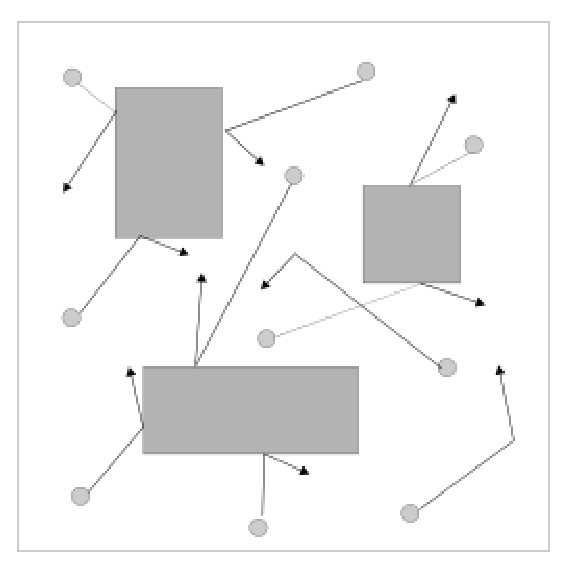
\includegraphics[scale=0.5]{./graph/OMM1}
\caption{Mobilo mezglu kustība laukumā ar šķēršļiem \cite{jabras}} \label{fig:omm1}
\end{minipage}%
\hspace{0.1cm}
\begin{minipage}[t]{0.49\linewidth}
\centering
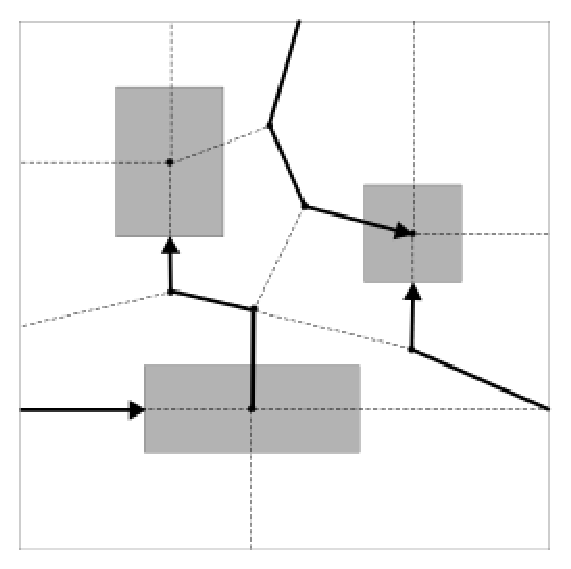
\includegraphics[scale=0.5]{./graph/OMM2}
\caption{OMM ar iepriekš noteiktiem kustības maršrutiem \cite{jabras}} \label{fig:omm2}
\end{minipage}
\end{figure}

Simulācijas rezultāti parāda, ka šķēršļu izmantošana un mezglu mobilitāte būtiski ietekmē ekspromta tīkla protokola veiktspēju \cite{jabras}.